\chapter{INTRODUCTION}\label{chap:intro}
This chapter explores the basics of heat transfer and molecular dynamics. The challenges existing in the current methods of finding transport quantities using molecular dynamics are included. Finally, applications of molecular dynamics to finiding thermal tranport in systems of interest are presented. The remaining chapters use the methods described here to examine systems of interest.

The first application, gold nanospheres of varying sizes and ligands, are presented in Chapter 2.  There are three different variables to characterize these systems: particle size, ligand length, and ligand rigidity. Through looking at the vibrational density of states and the density profiles for the systems, two important factors for heat transport can be determined: the vibrational overlap of the material at the interface and the physical proximity/overlap of the material at the interface. This information gives relevant principles for ligand and particle design, while no clear trend for particle radius was established. 

In an attempt to detangle the size and the ligand dependence, Chapter 3 takes a closer look at the particle surface and size dependence. 
The particles are left bare but have a range of sizes and three different geometries: spheres, icosahedra, and cuboctahedra.
The three different morphologies give  distinct vibrational spectra at the particle surface, allowing for different thermal conductivity. In addition to the particles, planar systems displaying the prominent facets of the particles were studied. This work suggests the need for a proximity factor contributing to a model of thermal transport.
The vibrational overlap of the material at the interface matters, but so does the amount of the material that is transferring heat. This is most clearly seen through the surface density of undercoordinated surface atoms in the planar systems.

Chapter 4 presents a combination of the concepts in the previous chapters through the study of small nanoparticles both in isolation and in a nanoarray. The $\ce{Au}_{144}\ce{PET}_{60}$ particle are approximately 9 \AA\ in radius and have a crystal structure found at very low temperatures which is an appropriate starting structure simulating heat transport in arrays. A unique aspect of these particles, and similar small structures, is that the ligand layer has gold atoms pulled away from the surface. This leads to lower coordination of the outer-most gold atoms, which now exhibit different vibrational spectra. These particles were simulated in two different solvents to observe solvent effects on the thermal conductivity of these particles.

Finally, Chapter 5 looks forward to potential applications of a new fluctuating charge embedded method to be applied to metal surfaces and particles in polarizable solvents. This new method would allow for the examination of charge effects on thermal transport and arrangement of solvent at the surface of the metal.

\section{Heat Transport}
The classical definition of temperature is a quantity that describes a thermal equilibration phenomena. At the macroscopic level, heat can be transferred in three ways: conduction, convection, and radiation.~~\cite{Chen2005} 
Under the equipartition theorem, where the average kinetic energy of a particle is \(\frac{3k_{B}T}{2}\), the temperature is a reporter of the kinetic energy of the system.~\cite{Goldstein2001}
When the kinetic energy is distributed evenly among all independent parts of the system, the heavy atoms in a system would have a small average speed than the lighter atoms in the system. 

On the microscopic level, heat moves through different paths depending on the composition of the system.~\cite{Chen2005}
In a gas, heat is transferred primarily through collisions, while in semiconductors thermal energy moves through the propagation of vibrations in the solid, ie. phonons. 
A phonon is a quantized lattice wave that traverses the material with a longitudinal or transverse polarization.~\cite{Kittel} 
In metals, where the material has a solid lattice embedded in a sea of electrons, both phonon and electron heat transfer contribute.~\cite{Kittel} 
Electrons in a metal system are typically treated as an electron gas.
Electrons travel at velocities that are approximately three orders of magnitude larger than phonons, therefore the electron contribution dominates heat transfer in metals and is important when considering bulk thermal conductance of metals.
At a metal/non-metal interface the thermal conductance through the non-metal is dominated by phonon scattering, rather than electronic contributions.~\cite{Chen2005, Cahill2011, Stoner1993}
%(All prior material is from Gang Chen Book)

\subsection{Heat Transfer at Interfaces}
Further examination of phonons as the only heat carriers can be done at the interface of two materials. If the phonon is traveling through material A and approaches material B with frequency $\omega$, with angles $\phi$ and $\theta$ normal to the interface; there is a transmission probability, $\tau_{a\rightarrow b}(\omega)$, that the wave will continue into material B (see Figure \ref{fig:interface-graphic}).~\cite{Monachon2016} 
The transmission probability must satisfy detailed balance.
%, meaning $\tau_{a\rightarrow b} = 1 - \tau_{b\rightarrow a}$
There are two major models that make predictions for heat transfer at the interface: the acoustic mismatch model (AMM) and the diffuse mismatch model (DMM).~\cite{Monachon2016}
\begin{figure}
    \centering
    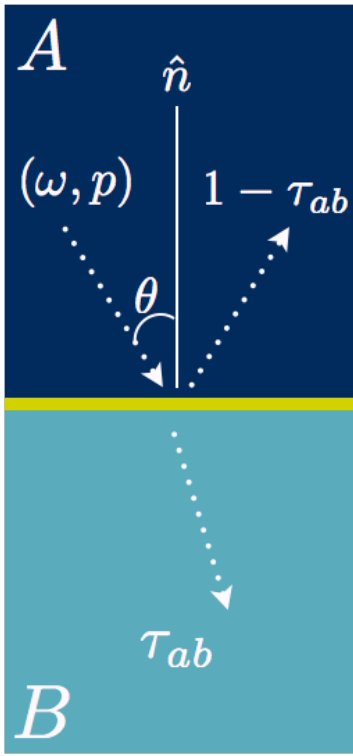
\includegraphics[scale=0.75]{figures/interface-graphic.png}
    \caption{Here an incoming phonon in material A is approaching the interface of materials A and B. The wave has a polarization ($p$) and frequency ($\omega$) and approaches the interface at an angle ($\theta$) relative to the normal of the interface. The phonon, under the DMM, has two options at the interface: scatter through to material B or scatter back through material A. The probability of transmission is given by $\tau_{ab}$. Due to detailed balance, the scattering back to material A is $1 - \tau_{ab}$.}
    \label{fig:interface-graphic}
\end{figure}

\subsection{Acoustic Mismatch Model}
In the acoustic mismatch model, the transmission probability- the total fraction of energy transmitted across the interface- is dependent on the acoustic impedance of the material, $Z_i$. The AMM evaluates the transmission coefficient through a continuum approach.~\cite{Little1959} This model uses the acoustic transmission and reflection between the two materials and ignores the granularity of the materials. Therefore the AMM would be most appropriate for low temperatures where the thermal spectrum is dominated by long wavelength phonons.~\cite{Graff1975} 

Each transmitted phonon has three possible polarizations: one longitudinal and two transverse. Likewise, reflected phonons can be reflected in the same fashion, giving six different paths for a wave to interact with the interface. This problem is usually simplified sing the acoustic analog of Snell’s law:
\begin{equation}
\tau_{ab}(\theta, p) = \frac{4\frac{p_2 \nu_{p, 2}}{p_1 \nu_{p,1}} \frac{\cos{\theta_{p,2}}}{\cos{\theta_{p,1}}}}{\big( \frac{p_2 \nu_{p, 2}}{p_1 \nu_{p,1}}+ \frac{\cos{\theta_{p,2}}}{\cos{\theta_{p,1}}}\big)^2}
\end{equation}
where $\theta$ are related to the analog of Snell's law through the frequency: \(\frac{\sin{\theta_1}}{\nu_1} = \frac{\sin{\theta_2}}{\nu_2}\).

Transmission can be simplified using acoustic impendances:
\begin{equation}
\tau_{ab}(\theta, p) = \frac{4Z_a Z_b}{(Z_a +Z_b)^2}
\end{equation}
where $Z$ is the acoustic impedance of each material, $Z_a = \rho_a v_a$, which depends on, $\rho$, the density and $v$, the speed of sound in the material. 

More complex treatments of the sound waves~\cite{Prasher2000} and treatments accounting for the interfacial bonding~\cite{Prasher2009} through the AMM have been studied. These modifications result in values that are lower than traditional AMM, therefore much below the experimental measurements of the systems.~\cite{Cahill2006, Stoner1993}

\subsection{Diffuse Mismatch Model}
The diffuse mismatch model assumes that the phonon has two options when the wave meets the interface: the phonon can transfer into material B or be reflected back into material A (see Figure \ref{fig:interface-graphic}). It operates under the assumption that all phonons at the interface are scattered randomly, meaning that all memory of the direction and polarization are lost. The phonon only keeps the frequency constant during the interaction of the two materials, hence all probability of the phonon to propagate into a material is dependent of the material's density of states. 

Under the DMM, the thermal conductance at an interface between $a$ and $b$ can be approximated,  
\begin{equation}
G_{ab} = \frac{1}{4 \pi} \sum_p \int_\omega \int_\theta \int_\phi \hbar \omega \frac{\partial f}{\partial T}  v_a  \rho_a  \tau_{ab} \cos\theta \sin\theta d\theta d\phi d\omega
\end{equation}
where $f$ is the Bose-Einstein distribution function, $v_a(\omega, p)$ is the group velocity (on side $a$) for a phonon characterized by frequency $\omega$, moving in direction ($\theta, \phi$) with polarization $p$.  The relevant material properties are the density of phonon states, $\rho_a(\omega, p)$, and the transmission probability, $\tau_{ab}(\omega, p)$, at the interface.~\cite{Swartz:1989uq,Reddy:2005fk,Monachon2016}  The DMM also assumes that phonons scatter into states with the same frequency on either side, and that the scattering phonons lose memory of their incident angles.  This requires a symmetry in the transmission probabilities,
\begin{equation}
\tau_{ab}(\omega) = 1 - \tau_{ba}(\omega)
\end{equation}

The DMM has a number of significant issues, particularly when the Debye model does a poor job representing the density of states, or where there is a fictitious boundary between identical materials (where the DMM predicts a non-zero resistance).~\cite{Monachon2016}  There is also an assumption of detailed balance built-in to the model,~\cite{Chen2005} which requires the two sides to be at equilibrium.
The DMM is more appropriate for modeling thermal transport at noncryogenic temperatures and at rough interfaces because the majority of acoustic phonons at $\geq$300 K have short wavelengths. The wavelengths at these temperatures are comparable to the interatomic spacing in the system.

While attempts to account for interfacial bonding have been made in the AMM, the DMM interfacial methods have not been developed.
The interaction of the materials at the interface has been found to be of significant importance to thermal conductivity~\cite{Beechem2007, Hopkins-surf-rough, Hopkins-inelastic}, but a factor to include this interaction has yet to be incorporated in the theory.
Despite the DMM's pitfalls, it has been the most commonly used model for the past 30 years. ~\cite{Cahill2006, Stoner1993, Stevens2005, Cahill2011}

\section{Molecular Dynamics}
Molecular dynamics is a computer simulation technique used to study structure and dynamics for atoms and molecules using classical mechanics. 
A simple algorithm of a molecular dynamics simulation can be described given atoms with initial positions and velocities, and forces (derived from potential energy surfaces described later) that are used to move the atoms. The time is incremented and the cycle repeats by calculating the forces (see Figure \ref{fig:MDschematic}). The atomic motion follows from Newton's equations of motion. The positions and velocities at each time step create a trajectory of the system that is time reversible. 

\begin{figure}
    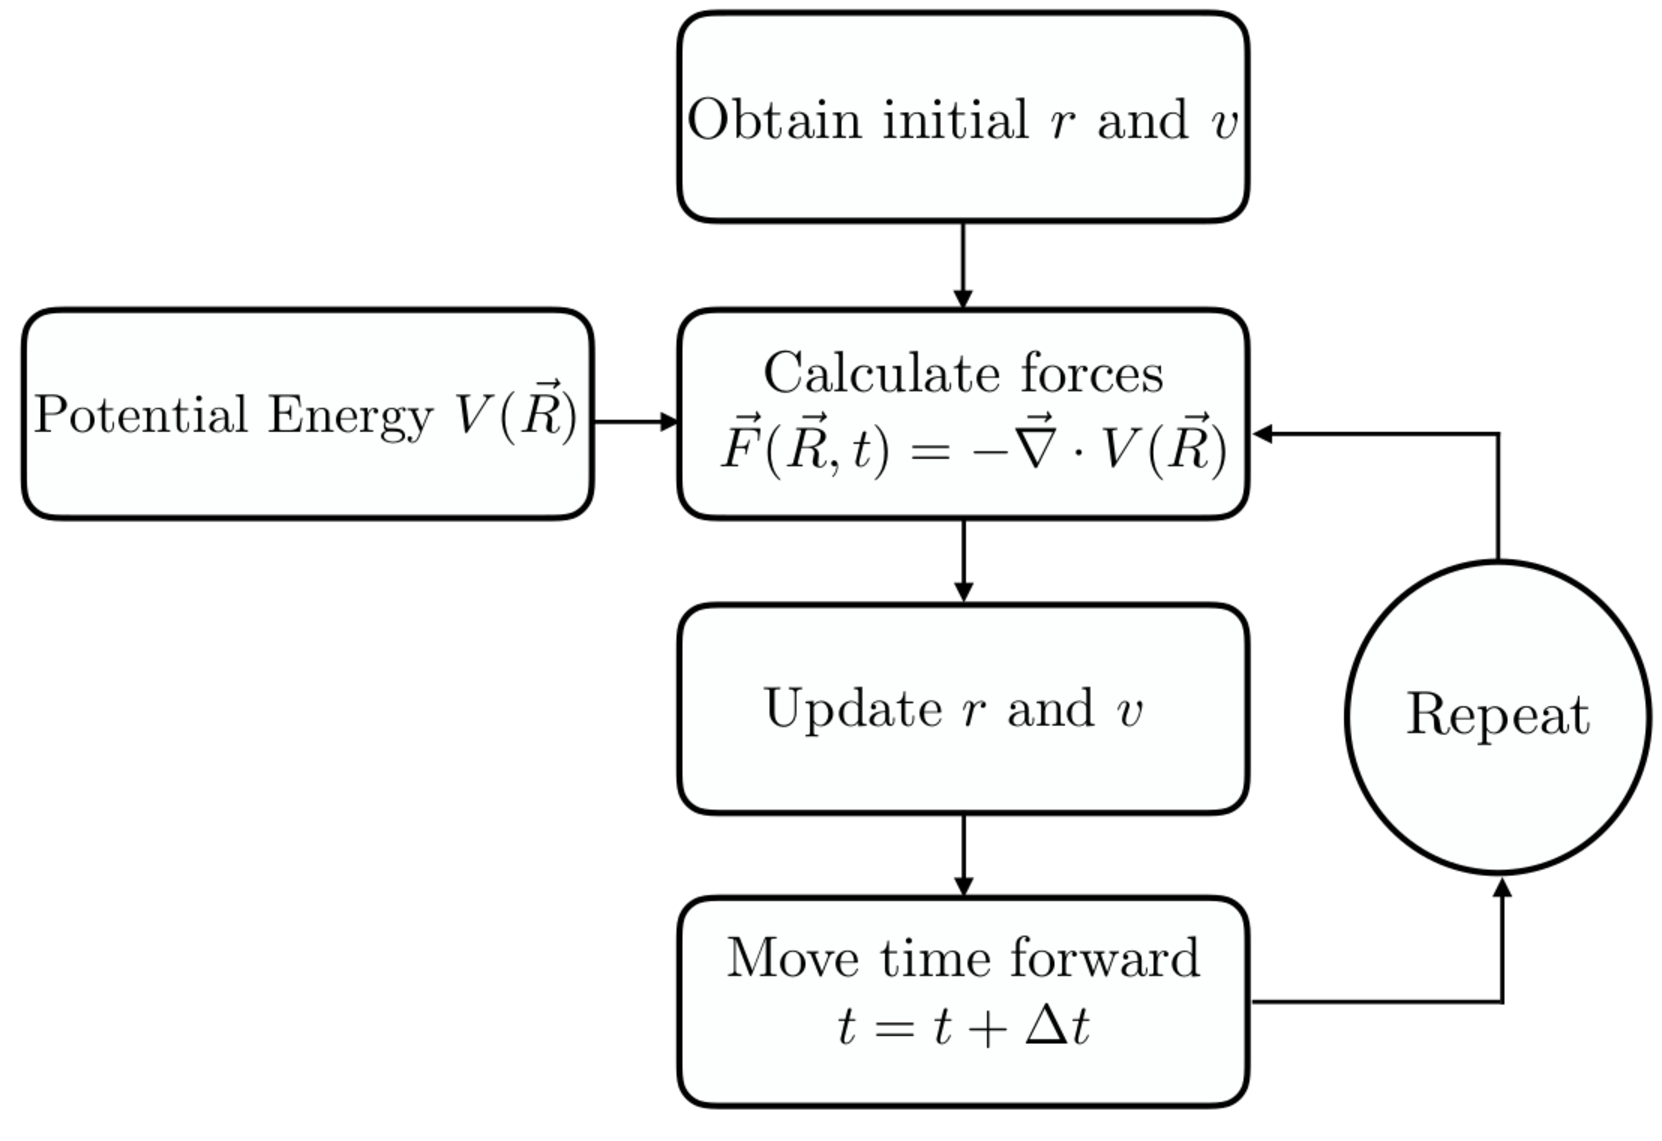
\includegraphics[scale=0.45]{figures/MDschematic.pdf}
    \caption{The initial positions, $r$, and velocities, $v$, are established in a system and from the potential energy, forces on the atoms is found. From the forces, positions can be changed then the velocities can be updated. The time can be moved forward and the process repeated at the calculated forces step until the desired time is reached.}
    \label{fig:MDschematic}
\end{figure}

Forces between each pair of atomic sites are computed from an interaction potential, where the forces are the gradient of the scalar potential:
\begin{equation}
\vec{F}(\vec{R},t) = -\vec{\nabla} \cdot V(\vec{R})
\end{equation}
These potentials are approximated using intra and inter molecular forces in the system to make an approximate potential energy surface with respect to the nuclear coordinates of the system.~\cite{Leach2001} 
\begin{equation}
   V(\vec{R}) = V_{bonded} + V_{electrostatic} + V_{vdW} + V_{metallic} +V_{constraints} + V_{hb}     
\end{equation}
The simplest of these to start with is the intra-molecular forces $V_{bonded}$, composed of bonds, bends, and torsions. Typical bonding potentials take the form of either harmonic bonds,
\begin{equation}
    V_{bond}(r) = \frac{k_{ij}}{2} (r - r_{ij}^0)^2
\end{equation}
or Morse bonds,
\begin{equation}
    V_{bond}(r) = D_{ij} [1 - \exp^{-\beta (r - r_{ij}^0)}]^2 .
\end{equation}
While other potential forms such as cubic and quartic can be used, the main form used in the following work will follow the harmonic form. In the harmonic form there are two variables that need to be provided: $k_{ij}$ and $r_{ij}^0$. The former is the spring constant associated with how the bond behaves when stretched and contracted. The latter is the equilibrium bond distance between the two atoms.

Similar to the bonding potentials, the bending potentials may take many forms. In this work, the harmonic potential,
\begin{equation}
    V_{bend} (\theta) = \frac{k_{ijk}}{2} (\theta - \theta_{ijk}^0)^2,
\end{equation}
was used, where $\theta$ is the angle between three connecting beads i, j, and k. $\theta_{ijk}^0$ is the equilibrium bend angle and $k_{ijk}$ is the spring constant for the bend.

The potential due to torsions within a bonded system is from the rotation of the plane made from the $i$, $j$, and $k$ points relative to the $l$ point:
\begin{equation}
    V_{torsions} (\phi_{ijkl})= c_1 [1 + \cos{\phi_{ijkl}}] + c_2 [1 + \cos{2\phi_{ijkl}}] + c_3 [1 + \cos{3\phi_{ijkl}}]  
\end{equation}
where the angle $\phi_{ijkl}$ is $(\hat{r}_{ij} \times \hat{r}_{jk}) \cdot (\hat{r}_{jk} \times \hat{r}_{kl})$ and $\hat{r}_{ab}$ is the unit vector between $a$ and $b$.


Inter-molecular,  or non-bonded interactions, are interactions between molecules which include the electrostatic interactions and van der Waals interactions, as well as metalic interactions.
The potential for electrostatic interactions
\begin{equation}
    V_{electrostatic} = \frac{q_i q_j}{4 \pi \epsilon_0 \mid r_{ij}\mid},
\end{equation}
describes the potential between two charged sites interacting via Coulomb's law.
Van der Waals interactions in this work are described via the Lennard Jones potential,
\begin{equation}
    V_{vdW} = 4\epsilon\bigg[\bigg(\frac{\sigma}{\mid r\mid}\bigg)^{12} + \bigg(\frac{\sigma}{\mid r\mid}\bigg)^6\big]
\end{equation}
where $\epsilon$ is the well depth when the distance between the two bodies is at the minimum and $\sigma$ is the distance the well starts from zero. 
The $\frac{1}{r^6}$ term is similar to dispersion and the $\frac{1}{r^{12}}$ term is empirically added to approximate repulsion due to electron exchange correltation.

The last, and one of the most important terms for the work is $V_{metallic}$. Quantum Sutton-Chen(qSC) potential is the metallic potential used in all the following projects.\cite{Qi:1999ph} The potential is broken into two parts: a pair potential and the local density accounting for cohension.
\begin{equation}
    V_{metallic} = \sum_i \epsilon \Bigg[ \sum_{j\neqi} V_{ij}^{pair} (r_ij) - c\sqrt{\rho_i}}\Bigg]
\end{equation}
\begin{equation}    
    V_{ij}^{pair} (r) = \bigg(\frac{a_{ij}}{r_{ij}}\bigg)^{n_{ij}}
\end{equation}
\begin{equation}
    \rho_i = \sum_{i\neq j}\bigg( \frac{a_{ij}}{r_{ij}}\bigg)^{m_{ij}}
\end{equation}
For gold, which is the only metal present in the following work the following values are used: $n=11$, $m=8$, $\epsilon=7.8052 x 10^-3$ eV, $c=53.582$, and $a=4.0651$ \AA.
$epsilon$ is the well well depth of the metallic interact and $a$ is the lattice parameter of the metal. qSC is the quantum corrected form of the Sutton-Chen potential.
Other common potential for metal interactions are Lennard-Jones and Embedded Atom Method (EAM).\cite{}

The last two terms in the full potential equation, $V_{constraints}$ and $V_{hb}$, hydrogen bonding, are not relevant to the simulations presented in this work.

\subsection{Representations of Atoms}
Molecular dyanamics is a lower accuracy method than first principals methods. There are different levels of simplification of the treatment of molecules.~\cite{Leach2001} 
Chiefly, there are three ways of treating the molecules in a given system that will be discussed here. 
The first, all-atom, is representing each atom within the system as a bead. In a molecule, these beads share bonds with atoms they are covalently bonded with and experiences bends and torsions within the larger molecule.

The next is a simplified version of the all-atom representation, united-atom, which compresses the hydrogen atoms onto the larger atom to which they were bonded. The mass and atomic radius of this bead is increased according to the number for hydrogens added.

United-atom calculations are faster due to the decrease in N, the number of atoms. They also are a better representation of heat transport. The vibrations of the molecules are of paramount importance in thermal transport and bonds to hydrogen have a high vibrational frequency. In molecular dynamics, the vibrational modes are occupied equally due to equipartition of the energy, thus the vibrational spectrum of the molecule will have high frequency \ce{C-H}, \ce{N-H}, or \ce{O-H} peaks. These high frequencies are irrelevant in most thermal transport calculations and thus all-atom simulations add expense and information that detracts from the low frequency picture of the system.

The last treatment discussed here is coarse-grained systems. These systems are further simplifications of the atoms present in the molecules. In coarse-grain systems, beads from the united atom model would be grouped into a single bead that represents a small molecule. The granularity of the beads can be adjusted from system to system and depends on the property desired and the timescale of the simulation. In general, coarse-graining is used widely for biologically relevant systems (i.e. proteins, lipids, etc.).
    
\subsection{Boundary Conditions}
In many simulations the desired quantity is a bulk property. To simulate a full bulk system would require too many atoms and too much time than possible within the lifetime of a graduate student. Further, the large box would have effects from the edges of the box. So how can the surface effects be avoided and simulate a bulk-like simulation?

\begin{figure}
    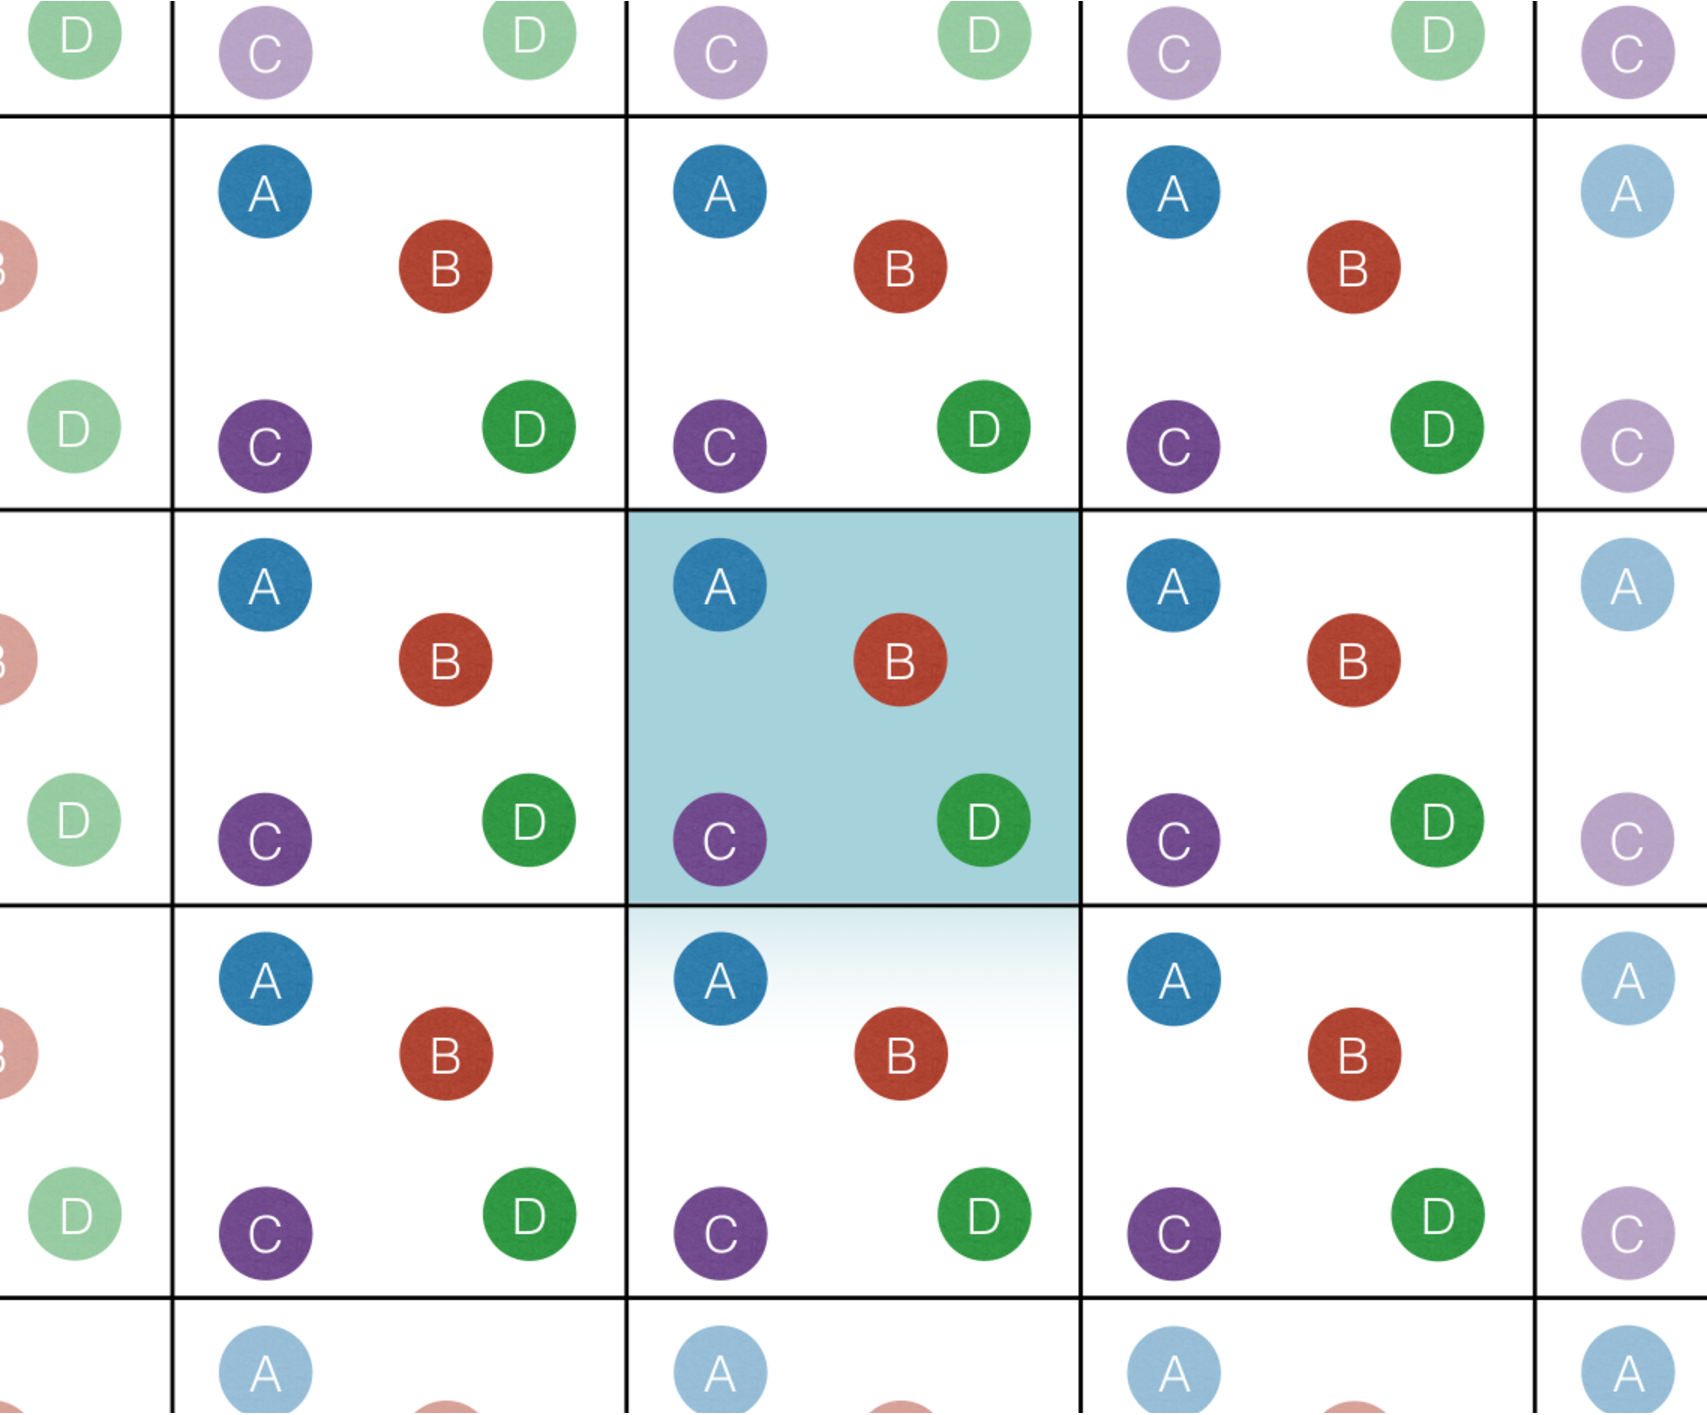
\includegraphics[scale=0.5]{figures/pbc-center.pdf}
    \caption{This figure is an example of periodic boundaries in two dimensions. Here the middle cell (colored square) is the system and each surrounding cell is an `image' of the original. As can be seen in the relation between particle A and C, sometimes the image particle provides the closest interaction or minimum image and would be within the cutoff radius when calculating interactions.}
    \label{fig:pbc}
\end{figure}

The above issues can be addressed with periodic boundary conditions. A simulation cell that has bulk-like density can reproduce bulk properties. Periodic boundary conditions are typically applied to orthorhombic simulation boxes, though any space filling geometry works. An `image' copy of the the simulation box is replicated in every direction. For example, in two dimensions periodic boundaries are represented in Figure \ref{fig:pbc}, where the simulation box has eight copies. In three dimensions, twenty-six images of the original box surround the simulation cell, for an orthorhombic box.
    
In a simulation, it is only necessary to track the particles in the central box.
The particles' images in neighboring cells are located at integer increments of the box dimension along each principal axis. 
So if the particle exits the right boundary of the cell, it will return in the box on the left boundary (from the neighboring simulation cell), which preserves the number density of the cell. 
In addition to periodic boundaries, the minimum image convention is used to make the simulation computationally tractable. A particle only interacts with the closest periodic image of another particle in the system. 
This convention requires a spherical cutoff, where a particle's non-bonded interactions with other particles end at a finite distance, $r$, from the particle which is less than half the length of the periodic box. This ensures that the particle sees one image of each particle and does not interacting with an image of itself. 

Though periodic boundaries allows for bulk properties to be found, it creates artificial periodicity in the system and might require an unreasonable system size due to the box structure. Later in this work, simulations of isolated particles are utilized to get single particle properties. 
These isolated systems use the Langevin Hull method. While there are several non-periodic methods that allow for a constant pressure, the Langevin Hull can handle heterogeneous mixtures of materials with different compressibilites.~\cite{Vardeman2011} This method is a modified version of Kohanoff, Caro, and Finnis' method for constant pressure and temperature non-periodic simulations based on Langevin dynamics.~\cite{Kohanoff:2005qm, Baltazar:2006ru} 

\begin{figure}
    \centering
    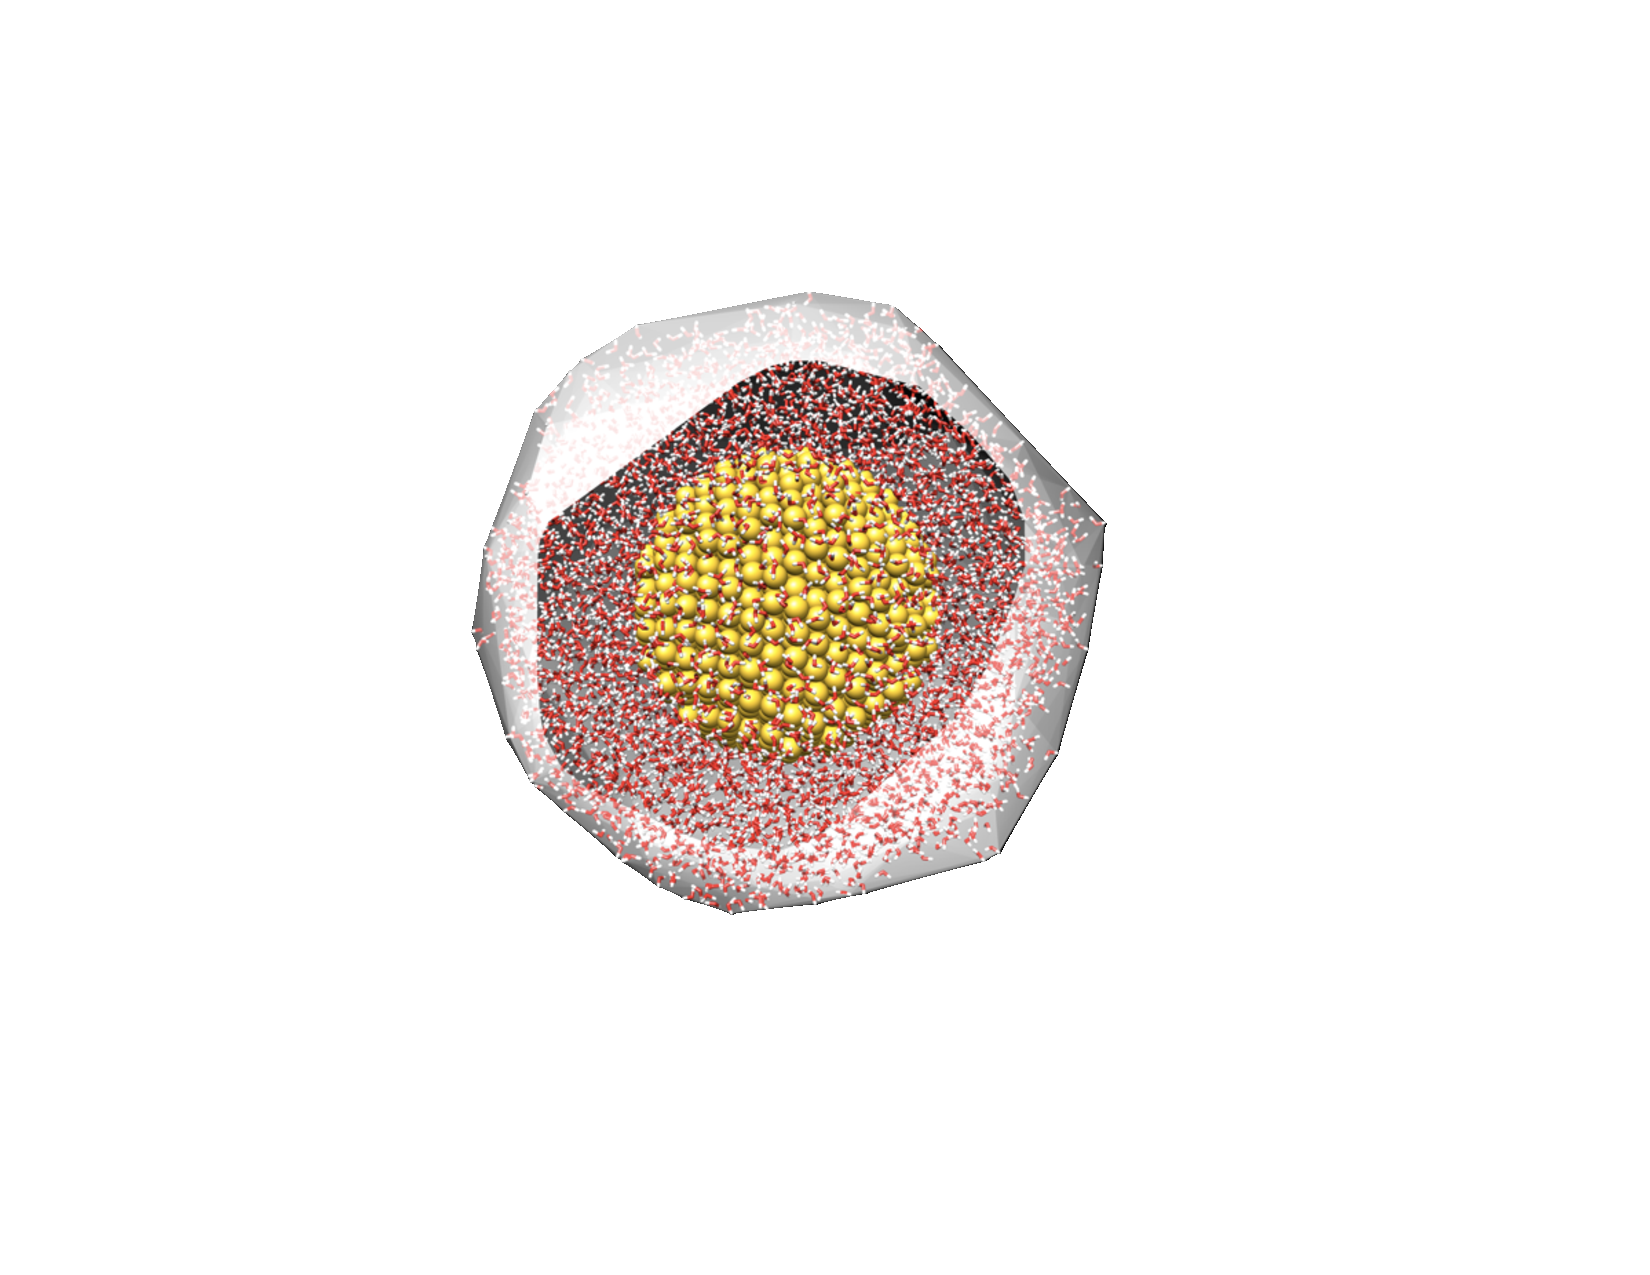
\includegraphics[scale=1]{figures/hull.pdf}
    \caption{Visualization of a gold particle solvated in water within the Langevin Hull taken from Vardeman \textit{et. al.}.~\cite{Vardeman2011}. The temperature and pressure bath interact with only the outer most atoms on the hull, the grey translucent surface. At each time step the hull is computed to ensure the atoms are interacting in the correct classifications, as edge atoms or as interior atoms.}
    \label{fig:hull}
\end{figure}

In the Langevin Hull method, the boundary of the system is a completely convex hull made of facets from points triangulated with the outermost atoms of the system. This hull interacts with a system bath that applies constant pressure and provides a thermal bath for the system through the facets of the hull. When looking at thermal properties of a system, the thermal coupling can be turned off to prevent artificial behavior due to the bath.

\section{Transport Coefficients}
Transport phenomena are controlled by the constitutive equations that describe how a material responds to various stimuli via transport.
The processes that are at the center of transport phenomena concern the transfer of mass, heat, or momentum. The transport of any of those listed would create a measurable flux in the system. The conservation equations conserve the desired property of interest in the presence of a flux.
The constitutive equations relate a transport property (diffusion, thermal conductivity, viscosity) to a flux via an empirical relationship. The flux, in all these cases, is proportional to the gradient and a constant of proportionality.

\begin{table}[h]
\centering
\caption{Constitutive and balance equations related to the transport coefficients of diffusivity, $D$, thermal conductivity, $\lambda$, and shear viscosity, $\eta$.  
\label{tab:coeff}}
\renewcommand*{\arraystretch}{2}
\begin{tabular}{ ccc }
\toprule
Transport & Constitutive & Balance\\
coefficients& equations& equations\\
\hline
$D$ & $\vec{j} = -D \cdot \vec{\nabla}c(\vec{r},t)$ & $\frac{\partial c(\vec{r},t)}{\partial t}+\vec{\nabla}\vec{j}=0$ \\
$\lambda$ & $\vec{q} = -\lambda \cdot \vec{\nabla}T(\vec{r},t)$ & $C_p \frac{\partial T(\vec{r},t)}{\partial t}+\vec{\nabla}\vec{q}=0$ \\
$\eta$ & $\sigma_{x,z} = -\eta \cdot \vec{\nabla_{z}}(\rho v_x)$ & $\rho \frac{D\vec{v}(\vec{r}, t)}{Dt}+\vec{\nabla} \overset{\leftrightarrow}{\sigma}=0$\\
\bottomrule
\end{tabular}
\end{table}
\begin{itemize}
    \item Diffusion (Fick’s Law):
$\vec{j} = -D \cdot \vec{\nabla}c(\vec{r},t)$

The diffusivity, $D$, or the diffusion coefficient is the proportionality between the concentration gradient of a species and the mass flux, $j$. 

\item Thermal Conductivity (Fourier’s Law):
$\vec{q} = -\lambda \cdot \vec{\nabla}T(\vec{r},t)$

The local heat flux density, $q$, is the produc of the conductivity of the material, $\lambda$, and the temperature gradient through the material. Therefore, $\lambda$ indicates the material's ability to conduct heat due to a temperature gradient. 

\item Viscosity (Newton’s Law of Viscosity): 
$\sigma_{x,z} = -\eta \cdot \vec{\nabla_{z}}(\rho v_x)$

The shear stress in the fluid, $\sigma$, is the product of the shear viscosity, $\eta$, and the perpendicular velocity gradient, $\vec{\nabla_{z}}(\rho v_x)$.

%\item Electrical Conductivity (Ohm's Law):
%$J = \sigma E$

%Where J, the current density at a point is equal to the electric field, E, at the same point by the material's electrical conductivity, $\sigma$.
\end{itemize}

All the transport coefficients ($D$, $\lambda$, $\eta$) describe how an instantaneous flux in a system relates to a corresponding gradient. Table \ref{tab:coeff} lists how the transport coefficients are involved in constitutive equations, where $\rho$ is the density and $C$ is the heat capacity of a material.

Transport phenomena are utilized in many fields, such as chemistry, physics, chemical engineering, electrical engineering, and mechanical engineering; to obtain the transport coefficients that describe a mechanical or chemical system. Atomistic simulations can provide insight for tuning experimental design. The three main ways to calculate transport coefficients, with a focus on thermal conductivity, will be discussed in detail in the following sections.

\subsection{Equilibruim Molecular Dynamics}
Transport properties from classical molecular dynamics simulations can be found using many methods. Equilibrium Molecular Dynamics (EMD) simulations use the most straightforward method. Under linear response theory, the transport coefficient can often be found using a relevant time correlation function to the transport coefficient of interest.~\cite{Heyes:1988ee,MASSOBRIO:1984bl,Helfand:1960os,Viscardy:2007rp,che:6888,kinaci:014106} In most cases either the Einstein relation or the Green-Kubo formulation are utilized to compute transport properties from the time correlation function in EMD.

The Einstein relation for thermal conductivity uses the Helfand moment, $G^\lambda (t)$, which is a centroid of the particle energies:
\begin{equation}
    G^\lambda (t) = \sum^{N}_{a=1} r_a (E_a - <E_a>)
\end{equation}
where $E_a$ is the energy of the particle $a$. Energy is given by the following: 
\begin{equation}
    E_a = \frac{p_a^2}{2m} + \frac{1}{2}\sum_{b\neq a} U(r_{ab})
\end{equation}
where $p_a$ is the momentum of $a$, $m$ is the mass, and $U(r_{ab})$ is the potential energy due to the presence of $a$.

The Einstein relation can  find the thermal conductivity using the fluctuations in the Helfand moment:
\begin{equation}
    \lambda = \lim_{N,V,t \rightarrow \infty} \frac{1}{2k_B T^2 Vt} \bigg< \Big[ G^\lambda (t) - G^\lambda (0) \Big]^2\bigg>
\end{equation}
where $k_B$ is the Boltzmann constant, $T$ is the temperature, $V$ is the volume, and $t$ is the time.

The equivalent Green-Kubo relation for thermal conductance is
\begin{equation}
    \lambda = \frac{1}{3Vk_BT^2}\int^\infty_0 dt <q(t) \cdot q(0)>
\end{equation}
where $q$ is the heat current.
The heat current can be found through
\begin{equation}
    q(t) = \sum^N_{i=1} E_i \vec{v_i} + \frac{1}{2}\sum_{j \neq i} \vec{r_{ij}} (f_{ij} \cdot \vec{v_j}).
\end{equation}
The first term is a summation of the energy times the velocity of all particles. The second term contains the force on atom $i$ due to atom $j$, $f_{ij}$.
In contrast to the Einstein relation where the mass, velocity, and potential are easily obtained from an equilibrium simulation, the heat current requires significantly more effort.

Both the Einstein and Green-Kubo relations for thermal conductiviy rely on correlation functions, where the long-time tails are able to significantly contribute to the integrated area and need long simulation times to achieve convergence.
The noise and poor convergence in the long-time tails give a poor estimation for the thermal conductivity and thus EMD simulations are not the best method for calculating this transport coefficient.
Moreover, these calculations have further complications when the systems contain an interface or are non-homogeneous.

\subsection{Non-Equilibruim Molecular Dynamics}
Since EMD has limitations due to the noise in the correlation function, methods in non-equilibrium molecular dynamics, NEMD, were developed that introduce a gradient into the simulations.~\cite{Backer:2005sf,Hess:2002nr,Picalek:2009rz, Vasquez:2004ty}
Typically these methods are used to impose a temperature or velocity gradient on a system to measure the corresponding transport coefficient. ~\cite{Evans:1982oq, Erpenbeck:1984qe, Evans:1986nx, Vogelsang:1988qv, Maginn:1993kl, Hess:2002nr, Schelling:2002dp, Berthier:2002ai, Evans:2002tg, Vasquez:2004ty, Backer:2005sf, Jiang:2008hc, Picalek:2009rz}
With linear response of a flux due to the applied gradient, the transport coefficient can be calculated using the constitutive equation: $J_z = -\lambda \frac{\partial T}{\partial z}$, where $\frac{\partial T}{\partial z}$ is imposed and $J_z$ is the resulting flux.
In NEMD, the temperature gradient is imposed by choosing sections of the simulation box to have particular temperatures. For example, a center portion of the system will be set to high temperature and the edges set to a lower temperature to impose the gradient. 
The imposed thermal gradient must be relatively small to maintain a linear relationship between the flux and the gradient. 
The corresponding transport coefficient, thermal conductivity, can be found if linear response holds.

Accurately measuring the thermal flux from the imposed gradient is difficult.
This method requires thermostats to maintain the thermal gradient which means that it does not ensure momentum or energy conservation and that simulations are restricted to the canonical ensemble.
Additionally, in heterogeneous systems, particularly with interfaces, it can be difficult to know what the shape of the imposed gradient should be at the boundaries of materials.

\subsection{Reverse Non-Equilibruim Molecular Dynamics}
Reverse non-equilibrium molecular dynamics (RNEMD) methods impose an unphysical flux and measure the gradient that develops.~\cite{Muller-Plathe:1997wq,Muller-Plathe:1999ao,Kuang:2012fe}
Imposed flux methods are preferable because the simulation imposes the difficult to measure quantity, the flux, causing the system to develop a gradient, which is easier to measure, between the regions where the flux is imposed. 
Since the measurement of a gradient is less complex, the imposed flux methods will typically take less time to obtain converged results, therefore the simulations are less time intensive and less costly.

The original RNEMD formulation imposes an artificial momentum flux between parallel slabs of material separated in the simulation cell. The flux was created by periodically swapping the momentum between molecules in each of the slabs in a homogeneous system.~\cite{Muller-Plathe:1997wq} 
This method was modified to obtain other transport coefficients ~\cite{Muller-Plathe:1999ao} and to handle heterogeneous systems.~\cite{Muller-plathe:2005} 
An attractive feature of RNEMD is that the algorithm conserves total linear momentum and total energy.
However, issues with large fluxes can result in non-linear gradients, where linear response can not be used to find the transport coefficient.~\cite{Tenney:2010rp}

This method has become widely used for thermal and mechanical properties of homogeneous and heterogeneous systems of solids and liquids~\cite{Muller-Plathe:1997wq,Muller-Plathe:1999ao, Tenney:2010rp}, as well as, interfaces.~\cite{Patel:2005zm, Shenogina:2009ix,Kuang:2011ef, Stocker:2013cl}
Gradients near interfaces exhibit distinct behavior at the boundaries of dissimilar materials.

Recent advances in RNEMD methodology have involved scaling particle velocities instead of swapping. The scaling method uses constraint equations that require the simulation to conserve total energy and total linear momentum.~\cite{Kuang:2011ef, Kuang:2012fe}
In addition, this RNEMD method has been extended to handle non-periodic heterogeneous systems.~\cite{Stocker:2014qq}

\section{Systems of Interest}
The systems that are explored in this work contain a solvated gold substrate or particle with heat transport from the gold to the solvent. 
Thermal properties of gold particles have been of great experimental interest, with a particular interest in detangling the important factors for transport: particle size,~\cite{Zanjani2014,Liu2015,Wilhelmsen2015,Stocker2016,Tascini2016} composition,~\cite{Wilson:2002uq, Ong:2013rt} surface modification,~\cite{kuang:AuThl,Ong:2013rt,Ong:2014yq,Liu2015,Stocker2016,Hannah2015,Park2016,Leitner2017} surface supports,~\cite{Park2012} exposed surface facets,~\cite{Hannah2015} and the chemical details of the environment.~\cite{Ge2006,Park2012,Ong:2013rt,Ong:2014yq,Wilhelmsen2015,Park2016} 

Three distinct studies examining interfacial thermal conductivity and heat transport will be explored with three different systems in this work.
The first system contains nanospheres with a range of particle radii and ligands with different length and rigidity.~\cite{Stocker2016}
The second system strips away the ligand layer and looks at bare particles with the intention of finding the role of in particle morphology.~\cite{Neidhart}
How exactly does the surface of the particle affect heat transport?
The third system looks at a more complex problem: how does the particle size and the system solvent change thermal conductivity of a nanoarray?
To simplify the atomistic models, we use a united-atom model for the ligand layer and solvent.
All the non-periodic systems use the Langevin Hull~\cite{Vardeman2011} and RNEMD methods for calculating transport properties.~\cite{Stocker:2014qq}
